\section{Closure with the Nearest particle statistics}

To circumvent this issue of diverging integral we introduce the \textit{Nearest neighbor statistic} in the form introduced \citet{zhang2021ensemble}. 
As the computation of the wake of the particle requires the knowledge of its velocity, we modify slightly the \textit{Nearest neighbor statistics} of \citet{zhang2021ensemble} to include a condition on the \textit{test } particle center of mass velocity.
Therefore, in the first place we introduce the \textit{Nearest neighbor velocity included} distribution as, 
\begin{equation}
    P_\text{nst}^f[\textbf{x},\textbf{r},\textbf{w},t]
    = \frac{1}{\phi_f}\avg{
        \chi_f[\textbf{x},t]
        \sum_i^N 
        \delta(\textbf{x}_i[\FF,t]-\textbf{y})
        \delta(\textbf{u}_i[\FF,t]-\textbf{w})
        h_i[\textbf{x},\FF,t]
    },
\end{equation}
where,
\begin{align}
    \label{eq:h_i_def}
    h_i[\textbf{x},\FF,t]
    = \frac{1}{N[\textbf{x},t,\FF]}
    \prod_j H(|\textbf{x}_j[\FF,t] - \textbf{x}| - |\textbf{x}_i[\FF,t] - \textbf{x}|)\\
    \label{eq:N_def}
    N[\textbf{x},t,\FF]
    = \sum_i\prod_jH(|\textbf{x}_j[\FF,t] - \textbf{x}| - |\textbf{x}_i[\FF,t] - \textbf{x}|).
\end{align}
It must be understood from this definition that $h_i=1$ if and only if the particle $i$ is the nearest neighbor to the point $\textbf{x}$. 
With that definition, $P_\text{nst}^f$ is the probability of finding the continuous the nearest neighbor of the point \textbf{x} located at \textbf{y} with a velocity \textbf{w} at time $t$, knowing that the continuous phase is present at \textbf{x}. 

By noticing that, 
\begin{equation}
    \int_{\mathbb{R}^6}
    \sum_i^N 
    \delta(\textbf{x}_i[\FF,t]-\textbf{y})
    \delta(\textbf{u}_i[\FF,t]-\textbf{w})
    h_i[\textbf{x},\FF,t]
    d\textbf{r}
    d\textbf{w} 
    =1,
\end{equation}
we arrive at the same conclusion as \citet{zhang2021ensemble} and write, 
\begin{equation}
    \avg{f_f^0\chi_f}
    = 
    \int_{\mathbb{R}^6}
    (f_f^\text{nst}P_\text{nst}^f\phi_f)[\textbf{x},\textbf{r},\textbf{w},t]
    d\textbf{r}
    d\textbf{w}
    \label{eq:ensemble_avg_to_nst}
\end{equation} 
where $f_f^0[\textbf{x},\FF,t]$ is an arbitrary property pertaining to the continuous phase, and $f_f^\text{nst}[\textbf{x},t|\textbf{w},\textbf{y}]$ is its conditional averaged on the presence of a nearest neighbor at \textbf{y} with velocity \textbf{w} and with the continuous phase at \textbf{x}, namely, 
\begin{equation}
    f_f^\text{nst}[\textbf{x},t|\textbf{w},\textbf{y}]
    =\frac{1}{(P_\text{nst}^f\phi_f) [\textbf{x},\textbf{r},\textbf{w},t]}
    \avg{
        (f_f^0
        \chi_f)[\textbf{x},t]
        \sum_i^N 
        \delta(\textbf{x}_i[\FF,t]-\textbf{y})
        \delta(\textbf{u}_i[\FF,t]-\textbf{w})
        h_i[\textbf{x},\FF,t]
    }.
    \label{eq:def_f_nst}
\end{equation}
Notice that the only difference between these definitions and the definitions presented in \citet{zhang2021ensemble}, i.e. Equation (2.6) to (2.8) of \citet{zhang2021ensemble}, is the inclusion of $\delta(\textbf{u}_i - \textbf{w})$ in our formulas. 
Anyhow, \ref{eq:ensemble_avg_to_nst} permitted us to express any ensemble averaged quantities in terms of \textit{Nearest neighbor conditioned} quantities. 
Therefore, this formula is in fact a tool similar to \ref{eq:batchlor_avg} but derived without any assumption, meaning with absence of errors. 

In the following we introduce the shorthand, 
\begin{equation*}
    \delta_\text{nst}^f [\textbf{x},\textbf{y},\textbf{w},t,\FF]
    =
    % \chi_f
    \sum_i^N 
    \delta(\textbf{x}_i[\FF,t]-\textbf{y})
    \delta(\textbf{u}_i[\FF,t]-\textbf{w})
    h_i[\textbf{x},\FF,t],
\end{equation*}
so that the conditional nearest neighbor average can simply be written, $f_f^\text{nst} P_\text{nst}^f \phi_f = \avg{\chi_f f_f^0 \delta_\text{nst}}$.

\subsection{A new Reynolds stress formulation}

Now, let us apply \ref{eq:ensemble_avg_to_nst} to the quantity of interest, specifically $f_f^0 = \textbf{u}_f'\textbf{u}_f'$, which yields: 
\begin{equation}
    \avg{\chi_f \textbf{u}_f'\textbf{u}_f'}
    = 
    \phi_f
    \int_{\mathbb{R}^6}
    \textbf{v}_f^\text{nst}
    \textbf{v}_f^\text{nst}
    P_\text{nst}^f
    d\textbf{y}
    d\textbf{w}
    + 
    \int_{\mathbb{R}^6}
    \avg{
        \chi_f
        \textbf{v}_f''
        \textbf{v}_f''
        % \sum_i 
        % \delta(\textbf{x}+\textbf{y}-\textbf{x}_i)
        % \delta(\textbf{w}-\textbf{u}_i)
        % h_i
        \delta_\text{nst}
    }
    d\textbf{y}
    d\textbf{w}
    \label{eq:relation_ensemble_nst}
\end{equation}
where we have defined: 
The fluctuation of the local value of the fluid phase velocity around the single particle conditional average $\textbf{v}_f'' = \textbf{u}_f^0 - \textbf{u}_f^\text{nst}$, and the fluctuation of the single particle nearest neighbor conditional average, around the ensemble average velocity, that is $\textbf{v}_f^\text{nst} = \textbf{u}_f^\text{nst} - \textbf{u}_f$. 
According to this definition, 
we state that we can separate the \textit{Reynolds stress} tensor into two distinct contributions :  (1) the agitation generated due to the averaged nearest neighbor averaged wakes around the particles at \textbf{y}, and (2) all other source of fluctuations such as those generated through particles interactions and the single phase turbulence. 
Notice that, this decomposition is similar than those used in \ref{eq:classic_avg} and \ref{eq:batchlor_avg}, the only difference is the presence of the \textit{nearest neighbor} averaged fields instead of the classic single-particle conditioned averaged fields. 

To give a better physical explanation of what is $\textbf{u}_f^\text{nst}$ we display on \ref{fig:unst} an instantaneous representation of the meaning of $\textbf{u}_f^\text{nst}$. 
\begin{figure}[h!]
    \centering
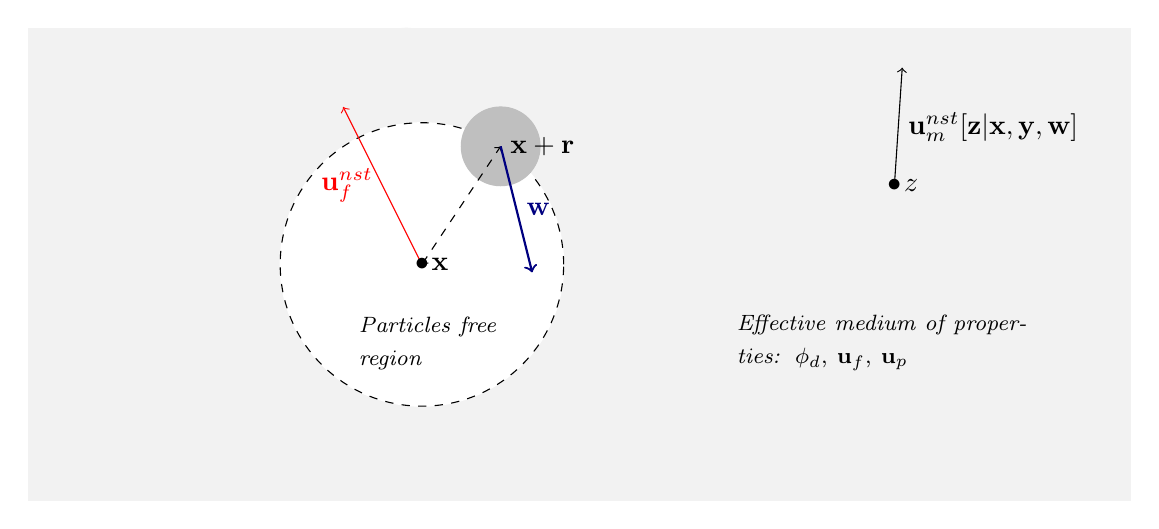
\begin{tikzpicture}
    \filldraw[gray!10](-5,-3) rectangle(9,3);
    \filldraw[white](0,0) circle (1.8);
    \filldraw[ gray!10!white](+2.6,0.5)circle (0.5);
    \filldraw[ gray!10!white](-1.5,2.2)circle (0.5);
    \draw[dashed](0:1.8) arc (0:360:1.8);
    % \filldraw[ gray!50!white](0,0) circle (0.5);
    \filldraw[ gray!50!white](1,1.5)circle (0.5);
    \filldraw[ gray!10!white](-0.2,2.5)circle (0.5);
    \draw[->,red](0,0)--++(-1,2)node[midway,left]{$\textbf{u}_f^\text{nst}$};
    \draw(0,0)node{$\bullet$}node[right]{$\textbf{x}$};
    \draw[dashed,<->](0,0)--(1,1.5)node[right]{$\textbf{x}+\textbf{r}$};
    \draw[->,blue!50!black,thick](1,1.5)--++(0.4,-1.6)node[midway,right]{$\textbf{w}$};
    % \draw[dashed](-0.2,3.5);
    \node[text width=2cm] (title) at (0.2,-1) {\footnotesize\textit{Particles free region}};
    % \node[ultra thick] (title) at (-0.5,-1.5) {(\textit{Case 1})};
    \node[text width=4cm] (title) at (6,-1) {\footnotesize\textit{Effective medium of properties:} $\phi_d$, $\textbf{u}_f$, $\textbf{u}_p$};
    \draw[->] (6,1)node{$\bullet$}node[right]{$z$}--++(0.1,1.5)node[right,midway]{$\textbf{u}_m^\text{nst}[\textbf{z}|\textbf{x},\textbf{y},\textbf{w}]$};
\end{tikzpicture} 
\caption{Representation of the \textit{nearest neighbor conditionally averaged} velocity fields $\textbf{u}_\text{nst}^f[\textbf{x},\textbf{w},\textbf{r},t]$, Inspired from (Figure 2) of \citet{zhang2021ensemble}}
\label{fig:unst}
\end{figure}
According to \ref{eq:def_f_nst} and \ref{fig:unst} $\textbf{u}_f^\text{nst}[\textbf{x},\textbf{r},\textbf{w}]$ is the averaged value of $\textbf{u}_f^0$, evaluated at \textbf{x}, on all configuration where a particle is present at $\textbf{y} = \textbf{x} + \textbf{r}$ with velocity $\textbf{w}$. 
Consequently, the region delimited by the sphere, centered at \textbf{x} of radius $|\textbf{y} - \textbf{x}|$ must be empty of particles center of mass \citep{zhang2021ensemble}. 
This deeper physical understanding will prove valuable in the subsequent section.  



\subsection{How to obtain the nearest neighbor conditional velocity fields ?}

In the objective of computing the sedimentation velocity, \citet[Appendix B]{zhang2021ensemble} has computed $\textbf{u}_f^\text{nst}$ using the \textit{nearest neighbor conditional averaged} Navier-Stokes equations. 
As his derivation does not provide detailed proof, especially on the derivation of Equation (B 1) of \citet{zhang2021ensemble},  we aim in this section to present a broader methodology. 

Inspired by the classic conditional average method of \citet{hinch1977averaged}, we stipulate that the nearest neighbor conditional velocity fields, i.e. $\textbf{v}_f^\text{nst}$,can be obtained by conditionally averaging the local scale mass and momentum equations, and solve for $\textbf{v}_f^\text{nst}$. 
Thus, let us first recall the local mass and momentum equation, 
\begin{align}
    \pddt (\rho_f\chi_f) +  \pddx \cdot (\rho_f\chi_f\textbf{u}^0_f) &= 0 \\
    \pddt (\rho_f\chi_f\textbf{u}^0_f)
    + \pddx\cdot (\rho_f\chi_f\textbf{u}^0_f\textbf{u}^0_f - \chi_f\bm\sigma^0_f)
    &= 
    - \delta_\Gamma \bm\sigma_f^0 \cdot \textbf{n}_d. 
    + \chi_f \rho_f \textbf{g}
    \label{eq:local_equations}
\end{align}
Then, note that we can obtain $\textbf{v}_f^\text{nst}$ from $\textbf{u}_f^0$ directly by the operation, 
\begin{equation*}
    \textbf{v}_f^\text{nst} P_\text{nst}^f
    = 
    \textbf{u}_f^\text{nst} P_\text{nst}^f
    - \textbf{u}_f P_\text{nst}^f
    = 
    \avg{\delta_\text{nst}^f \chi_f \textbf{u}_f^0}
    - \textbf{u}_f P_\text{nst}^f
\end{equation*}
We deduce that to obtain an equation for $\textbf{u}_f^\text{nst}$ we must multiply, \ref{eq:local_equations} by $\delta_\text{nst}$ and average overall configurations. 
This introduces the need of proper conservation equation for $\delta_\text{nst}$. 

\subsubsection{Conditionally mass transport equation}
Consequently, we introduce the  conservation equation of each distribution present in $\delta_\text{nst}$, it reads, 
\begin{align}
    \label{eq:dt_delta_x}
    \pddt \delta(\textbf{x}_i  - \textbf{y})
    +\textbf{u}_i  
    \cdot \pddy \delta(\textbf{x}_i  - \textbf{y})
    = 0\\
    \pddt \delta(\textbf{u}_i -\textbf{w})
    +\textbf{a}_i \cdot  \pddw   \delta(\textbf{u}_i  - \textbf{w})
    = 0\\
    \pddt \chi_f 
    + \textbf{u}_\Gamma^0 
    \cdot \pddx \chi_f = 0 \\
    \pddx \chi_f = - \delta_\Gamma \textbf{n}_f,
    \label{eq:chi_f_dt}
\end{align}
where we recall that $\textbf{u}_\Gamma^0$ is the velocity of the droplets interfaces, and $\textbf{n}_f$ is the normal pointing inward the droplets surfaces. 
Additionally, The vector $\textbf{a}_i$ correspond to the center of mass acceleration of the particle $i$. 
Form \ref{eq:dt_delta_x} to \ref{eq:chi_f_dt} we deduce that, 
\begin{align}
    \pddt \delta_\text{nst}
    + \pddy \cdot (\textbf{w} \delta_\text{nst})
    + \pddw \cdot (\textbf{a}_i  \delta_\text{nst})
    = 
    \sum_i \delta(\textbf{x}_i -\textbf{y}) \delta(\textbf{u}_i - \textbf{w}) \pddt h_i
\end{align}
% and, 
% \begin{align*}
%     \pddt (\chi_f \delta_\text{nst})
%     + \pddy \cdot (\textbf{w} \chi_f \delta_\text{nst})
%     + \pddw \cdot (\textbf{a}_i  \chi_f \delta_\text{nst})
%     = 
%     \chi_f \delta(\textbf{x}_i -\textbf{y}) \delta(\textbf{u}_i - \textbf{w}) \pddt h_i
%     + \delta_\Gamma \delta_\text{nst} \textbf{u}_\Gamma\cdot \textbf{n}_f
% \end{align*}
As, shown in appendix, 
\begin{align}
    \pddt  h_i[\textbf{x},t,\FF]
    = 
    h_i
    \sum_k 
    \delta(r_k - r_i)
    (\textbf{u}_k  \cdot \hat{\textbf{r}}_k - \textbf{u}_i  \cdot \hat{\textbf{r}}_i)\\
    \pddx  h_i[\textbf{x},t,\FF]
    = 
    h_i
    \sum_k 
    \delta(r_k - r_i)
    ( \hat{\textbf{r}}_k -  \hat{\textbf{r}}_i),
\end{align}
where we recall that $\textbf{u}_k$ and $\textbf{u}_i$  are the center of mass velocity of the particle $k$ and $i$ respectively.
Note that the second expression is in agreement with \citet[Appendix A]{zhang2021ensemble}. 
We also introduced the radial distance from the particle $i$ to the point $\textbf{x}$ namely, $r_i = |\textbf{x}_i - \textbf{x}|$.  
Anyhow, considering this relation yields a new expression for the transport equation of $\delta_\text{nst}$ namely,
\begin{equation}
    \pddt \delta_\text{nst}
    + \pddy \cdot (\textbf{w} \delta_\text{nst})
    + \pddw \cdot (\textbf{a}_i  \delta_\text{nst})
    = 
    % \sum_i
    % \delta(\textbf{x}_i -\textbf{y}) 
    % \delta(\textbf{u}_i - \textbf{w}) 
    \delta_\text{nst}
    % h_i
    \sum_k 
    \delta(r_k - r_i)
    (\textbf{u}_k  \cdot \hat{\textbf{r}}_k - \textbf{u}_i  \cdot \hat{\textbf{r}}_i). 
    % \label{eq:dt_delta_nst}
\end{equation}
As demonstrated in \citet{zhang2023evolution}, in another context, the right-hand side term of \ref{eq:dt_delta_nst} can be considered as a source term due to the birth or death of nearest neighbor to the point \textbf{x}. 
For reason that will become clear latter on we add the term $\textbf{u}_f^0\cdot \pddx \delta_\text{nst}$ on each side of the equation, which gives,
\begin{equation}
    \pddt \delta_\text{nst}
    + \textbf{u}_f^0\cdot \pddx \delta_\text{nst}
    + \textbf{w}   \cdot \pddy \delta_\text{nst}
    + \textbf{a}_i \cdot \pddw   \delta_\text{nst}
    = 
    % \sum_i
    % \delta(\textbf{x}_i -\textbf{y}) 
    % \delta(\textbf{u}_i - \textbf{w}) 
    \delta_\text{nst}
    % h_i
    \sum_k 
    \delta(r_k - r_i)
    ((\textbf{u}_k - \textbf{u}_f^0) \cdot \hat{\textbf{r}}_k - (\textbf{u}_i  - \textbf{u}_f^0)\cdot \hat{\textbf{r}}_i). 
    \label{eq:dt_delta_nst}
\end{equation}
On the right-hand side we have reformulated the term $\textbf{u}_f^0\cdot \pddx \delta_\text{nst}$, see \tb{Annexe} for the full derivation. 

To derive an equation for $P_\text{nst}^f$ we multiply \ref{eq:dt_delta_nst} by $\chi_f$, and make use of \ref{eq:chi_f_dt}, yielding, 
\begin{multline}
    \pddt (\chi_f\delta_\text{nst})
    +  \pddx \cdot (\textbf{u}_f^0 \chi_f\delta_\text{nst})
    +  \pddy \cdot (\textbf{w}    \chi_f\delta_\text{nst})
    +  \pddw \cdot   (\textbf{a}_i  \chi_f\delta_\text{nst})\\
    = 
    % \sum_i
    % \delta(\textbf{x}_i -\textbf{y}) 
    % \delta(\textbf{u}_i - \textbf{w}) 
    (\chi_f\delta_\text{nst})
    % h_i
    \sum_k 
    \delta(r_k - r_i)
    ((\textbf{u}_k - \textbf{u}_f^0) \cdot \hat{\textbf{r}}_k - (\textbf{u}_i  - \textbf{u}_f^0)\cdot \hat{\textbf{r}}_i). 
    \label{eq:dt_delta_nst_f}
\end{multline}
which upon averaging gives directly,
\begin{multline}
    \pddt (\phi_fP_\text{nst}^f)
    + 
    \pddx \cdot (
        \phi_f 
        P_\text{nst}^f
        \textbf{u}_f^\text{nst}
    )
    + \pddy \cdot (
        \phi_f
        P_\text{nst}^f
        \textbf{w} 
    )
    +
    \pddw \cdot (  
        \phi_f 
        P_\text{nst}^f
        \textbf{a}_p^\text{nst} 
    )
    = \\
    + \avg{
    %  \chi_f \textbf{u}_\Gamma \cdot \pddx \delta_\text{nst}
     \chi_f \delta_\text{nst}
    \sum_k 
    \delta(r_k - r_i)
    [(\textbf{u}_k - \textbf{u}_\Gamma^0) \cdot \hat{\textbf{r}}_k - (\textbf{u}_i- \textbf{u}_\Gamma^0)  \cdot \hat{\textbf{r}}_i]}.
    \label{eq:dt_P_nst_chi}
\end{multline}
where we have noticed that $\textbf{u}_\Gamma^0 = \textbf{u}_f^0$ in the absence of mass transfer. 
In this relation the left-hand side terms represent the advection of $\phi_f P_\text{nst}^f$.
The source term on the right-hand side of \ref{eq:dt_delta_nst_chi} accounts for the changes in nearest neighbor distribution due to the permutation of the nearest neighbor at the local scale. 
Notice the similarities of the right-hand side source term of \ref{eq:dt_delta_nst_chi} with (A10) of \citet{zhang2023evolution}, which derived a transport equation for $P_\text{nst}$ such as it is defined in the previous chapters. 
We remark that the source terms of (A10) and \ref{eq:dt_delta_nst_chi} yield the same form, but in \ref{eq:dt_delta_nst_chi} the velocity $\textbf{u}_i$ and $\textbf{u}_k$ are evaluated with respect to the local velocity of the fluid $\textbf{u}_f^0$, while in \citet{zhang2023evolution} it is evaluated relative to the velocity of the particles centered at \textbf{x}. 
This is not surprising considering the difference in definition between $P_\text{nst}^f$ and $P_\text{nst}$ in \citet{zhang2023evolution}. 


\ref{eq:dt_P_nst_chi} which can also be written in ``conservative'' form using \ref{eq:dt_P_nst_chi} and, 
\begin{equation}
    \pddt \phi_f 
    + \div(
        \phi_f
        \textbf{u}_f 
        ) 
    = 0, 
\end{equation}
to show that \ref{eq:dt_delta_nst_chi} can be written in ``conservative'' form, yielding, 
\begin{multline}
    \pddt P_\text{nst}^f
    + 
    \pddx \cdot (
        P_\text{nst}^f
        \textbf{u}_f^\text{nst}
    )
    + \pddy \cdot (
        P_\text{nst}^f
        \textbf{w}
    )
    +
    \pddw \cdot (  
        P_\text{nst}^f
        \textbf{a}_p^\text{nst} 
    )
    = \\
    + \frac{1}{\phi_f}\avg{
    %  \chi_f \textbf{u}_\Gamma \cdot \pddx \delta_\text{nst}
     \chi_f \delta_\text{nst}
    \sum_k 
    \delta(r_k - r_i)
    [(\textbf{u}_k - \textbf{u}_\Gamma^0) \cdot \hat{\textbf{r}}_k - (\textbf{u}_i- \textbf{u}_\Gamma^0)  \cdot \hat{\textbf{r}}_i]}.
    \label{eq:dt_Pc_nst_chi}
\end{multline}
This equation multiplied by $\rho_f$ corresponds to the \textit{nearest neighbor conditional averaged} mass equation of the fluid phase. 

\subsubsection{First form of the conditional averaged momentum equaiton}
Now that the transport equation for $\delta_\text{nst}$ and $P_\text{nst}^f$ are properly derived we are able to derive the \textit{nearest neighbor conditionally averaged} momentum equation. 
Multiplying \ref{eq:local_equations} by $\delta_\text{nst}$ , making use of \ref{eq:dt_delta_nst} and averaging overall configurations yields, 
\begin{multline}
    \pddt (\rho_f\phi_f P_\text{nst} \textbf{u}^\text{nst}_f)
    + \pddx\cdot (
        \rho_f\phi_fP_\text{nst}^f \textbf{u}^\text{nst}_f\textbf{u}^\text{nst}_f 
        +\bm\sigma_\text{nst}^\text{eq})
    + \pddy\cdot (\phi_fP_\text{nst}^f \textbf{w}\textbf{u}_f^\text{nst} )
    + \pddw\cdot (\phi_fP_\text{nst}^f \textbf{a}_p^\text{nst} \textbf{u}_f^\text{nst} )\\
    = 
    \phi_fP_\text{nst}^f  \rho_f \textbf{g}
    - \avg{\delta_\text{nst}\delta_\Gamma \bm\sigma_f \cdot \textbf{n}_d} 
    % - \avg{\chi_f \bm\sigma_f^0 \cdot \grad\delta_\text{nst}}
    +\avg{
        \delta_\text{nst}
        \chi_f \bm\sigma_f^0 \cdot
        \sum_k 
        \delta(r_k - r_i)
        [\hat{\textbf{r}}_k - \hat{\textbf{r}}_i]}\\
    +\avg{
        %  \chi_f \textbf{u}_\Gamma \cdot \pddx \delta_\text{nst}
         \textbf{u}_f^0\chi_f \delta_\text{nst}
        \sum_k 
        \delta(r_k - r_i)
        [(\textbf{u}_k - \textbf{u}_f^0) \cdot \hat{\textbf{r}}_k - (\textbf{u}_i- \textbf{u}_f^0)  \cdot \hat{\textbf{r}}_i]},
    \label{eq:momentum_avg_nst}
\end{multline}
with the effective stress $\bm\sigma_\text{nst}^\text{eq}$ defined as, 
\begin{equation}
    \bm\sigma_\text{nst}^\text{eq}=
    \avg{\rho_f\chi_f\delta_\text{nst} \textbf{u}''_f\textbf{u}''_f} 
    - \phi_f P_\text{nst}^f \bm\sigma^\text{nst}_f. 
\end{equation}
The terms on the left-hand side of \ref{eq:momentum_avg_nst} represents the advection of the \textit{nearest neighbor conditional average} momentum along the phase space coordinate, plus the contribution of the \textit{nearest neighbor conditional average} viscous stresses $\bm\sigma^\text{nst}_f$
The first term on right-hand side of \ref{eq:momentum_avg_nst} corresponds to the momentum exchange between phases, but conditionally averaged. 
The second and third terms are the additional contribution of the convective and non-convective fluxes due to the birth or death of nearest neighbors. 

In this form \ref{eq:momentum_avg_nst} is hardly solvable. 
Although boundary condition are available at the surface of our particle, for the velocity $\textbf{u}_f^\text{nst}[\textbf{y}+a \textbf{n}, \textbf{y},\textbf{w}]$ there is a lake of boundary condition infinitely far from the particle. 
Indeed, in this form $\lim_{|\textbf{x}- \textbf{y}|\to \infty} \textbf{u}^\text{nst}_f = \text{Undefined}$ because in the same limits $P_\text{nst}^f = 0$. 

\subsubsection{Second form of the conditional averaged equation}

To settle this issue we follow \citet[Appendix B]{zhang2021ensemble} and propose to solve for an auxiliary problem which is equivalent to the conservation equation of $\textbf{u}_f^\text{nst}[\textbf{x},\textbf{y},\textbf{w},t]$. 
We introduce the conditionally averaged fields, 
\begin{equation*}
    P_\text{nst}^f[\textbf{y},\textbf{w},\textbf{x},t]\textbf{u}^\text{nst}[\textbf{z},t|\textbf{x},\textbf{y},\textbf{w}]
    = \avg{\delta_\text{nst}^f  \textbf{u}^0[\textbf{z},\FF,t]}
    \label{eq:def_u_z}
\end{equation*}
where, $\delta_\text{nst}^f = \chi_f[\textbf{x},t,\FF]\delta_\text{nst}[\textbf{y},\textbf{w}, \FF,t]$. 
Additionally, we modified slightly the definition of $P_\text{nst}^f$, such that our new definition  is $\phi_f$ times the previous definition made in the preceding section, $P_\text{nst}^f[\textbf{x},\textbf{y},\textbf{w},t] = \phi_f[\textbf{x},t]P_\text{nst}^f[\textbf{y},\textbf{w},t|\textbf{x}]$. 
% With that definition, $\phi_f^\text{nst}$ is the fluid \textit{nearest neighbor conditionally averaged} fluid phase volume fraction, such that $\phi_f^\text{nst}$ represents the fluid phase volume fraction evaluated at \textbf{z} averaged on all configurations where \textbf{x} is occupied by the fluid phase and $\textbf{y}$ by a particle center of mass, with velocity $\textbf{w}$.  
$\textbf{u}^\text{nst}$ is the \textit{nearest neighbor conditionally averaged} velocity evaluated at $\textbf{z}$, knowing the fluid phase is also present at $\textbf{x}$ with the nearest neighbor to \textbf{x} being located in \textbf{y} with velocity \textbf{w}. 
A graphical representation of $\textbf{u}^\text{nst}$ is given \ref{fig:unst}.
With that definition we have the following boundary condition far from the particle free region, 
\begin{align*}
    \lim_{|\textbf{z} - \textbf{y}|\to \infty}
    \textbf{u}^\text{nst}[\textbf{z},t|\textbf{x},\textbf{y},\textbf{w}]
    = \textbf{u}[\textbf{z},t]
    % \lim_{|\textbf{z} - \textbf{y}|\to \infty}
    % \phi^\text{nst}[\textbf{z},t|\textbf{x},\textbf{y},\textbf{w}]
    % = \phi[\textbf{z},t],
    \label{eq:boundary}
\end{align*}
since far from the particle free region the effect of the particle located at \textbf{y} has no impact on the averaged quantities. 
Thus, $\textbf{u}^\text{nst}$ has the advantage of having proper boundary condition at infinity and is related to $\textbf{u}_f^\text{nst}$ such that, $\textbf{u}^\text{nst}[\textbf{x},t|\textbf{x},\textbf{y},\textbf{w}] = \textbf{u}_f^\text{nst}[\textbf{x},t|\textbf{y},\textbf{w}]$ since only the fluid phase is present at \textbf{x} by definition of $\textbf{u}^\text{nst}$. 

We also introduce the disturbance fields $\textbf{v}^\text{nst} = \textbf{u}^\text{nst} - \textbf{u}$, which follows the condition at infinity, 
\begin{equation}
    \lim_{|\textbf{z} - \textbf{y}|\to \infty}
    \textbf{v}^\text{nst}[\textbf{z},t|\textbf{x},\textbf{y},\textbf{w}]
    = 0,
\end{equation}
while the boundary condition at the surface of the particle is given by, 
\begin{equation}
    \textbf{v}^\text{nst}\cdot \textbf{n}
    = 
    (\textbf{w} - \textbf{u}[\textbf{z},t])\cdot \textbf{n}
    = 
    \left\{
        \textbf{w}
        - \textbf{u}
        - (\textbf{y} - \textbf{z})\cdot \grad\textbf{u}
        + \ldots 
    \right\}
    \;\;\; \forall \textbf{z}\in \left\{ |\textbf{z} - \textbf{y}| = a  \right\}. 
    \label{eq:bounday2}
\end{equation}
Notice that these boundaries conditions and the one derived in \ref{chap:daniel2} for the \textit{Single-point conditionally averaged} Navier-Stokes equations  are exactly the same but applied on the bulk velocity rather than on the continuous phase velocity.

Instead of using the fluid phase formulation of the mass and momentum local conservation equations, \eqref{eq:local_equations}, we use the \textit{single-fluid}, mass and momentum equations, namely, 
\begin{align}
    \pddz \cdot \textbf{u}^0 = 0 \\
    \pddt (\rho^0\textbf{u}^0_f)
    + \pddz\cdot 
    (\rho^0\textbf{u}^0\textbf{u}^0 
    -\bm\sigma^0)
    &= 
    + \rho^0 \textbf{g}. 
    \label{eq:local_equations_bulk}
\end{align}
Multiplying these equations by $(\delta_\text{nst}^f - P_\text{nst}^f)$ and averaging overall configurations yields the Navier-Stokes equations for the distance fields $\textbf{v}^\text{nst}$, namely,
\begin{equation}
    \pddz \cdot \avg{(\delta_\text{nst}^f - P_\text{nst}^f) \textbf{u}^0}
    = 0,
    \label{eq:mass_nst_d}
\end{equation}
and,
\begin{multline}
    \pddt \avg{(\delta_\text{nst}^f - P_\text{nst}^f)\rho^0\textbf{u}^0}
    + \pddz\cdot \avg{ (\delta_\text{nst}^f - P_\text{nst}^f) ( \rho^0  \textbf{u}^0 \textbf{u}^0 - \bm\sigma^0)}\\
    +  \pddx \cdot \avg{(\delta_\text{nst}^f \textbf{u}_f^0 - P_\text{nst}^f\textbf{u}_f^\text{nst}) \rho^0 \textbf{u}^0}
    +  \pddy \cdot \avg{(\delta_\text{nst}^f - P_\text{nst}^f) \textbf{w} \textbf{u}^0 \rho^0}
    +  \pddw \cdot \avg{(\delta_\text{nst}^f \textbf{a}_i - P_\text{nst}^f \textbf{a}_p^\text{nst})\textbf{u}^0 \rho^0 }\\
    = 
    % - \avg{(\delta_\text{nst}^f - P_\text{nst}^f)\delta_\Gamma \bm\sigma_f^0 \cdot \textbf{n}_d }
    + \avg{(\delta_\text{nst}^f - P_\text{nst}^f)\rho^0 \textbf{g}} 
    + 
    \avg{\rho^0 \textbf{u}^0 S'_\text{nst} },
    \label{eq:momentum_nst_d}
\end{multline}
where we have defined $S_\text{nst}'$ as the source term due to the interchanges of the nearest particles,
\begin{multline}
    S_\text{nst}'
    =
    \left\{
    \delta_\text{nst}^f
        % h_i
        \sum_k 
        \delta(r_k - r_i)
        ((\textbf{u}_k - \textbf{u}_f^0) \cdot \hat{\textbf{r}}_k - (\textbf{u}_i  - \textbf{u}_f^0)\cdot \hat{\textbf{r}}_i) 
    - \right.\\ \left.
    \avg{
         \delta_\text{nst}^f
        % h_i
        \sum_k 
        \delta(r_k - r_i)
        ((\textbf{u}_k - \textbf{u}_f^0) \cdot \hat{\textbf{r}}_k - (\textbf{u}_i  - \textbf{u}_f^0)\cdot \hat{\textbf{r}}_i) 
    }
    \right\}. 
\end{multline}
In this quite general form these equations may seem complicated, therefore let us describe in details the meaning of each term. 
We start by the conditional ``mass'' conservation equation \eqref{eq:mass_nst_d}. 
The term within the divergence sign can be written,  
\begin{equation}
    \avg{(\delta_\text{nst}^f - P_\text{nst}^f )\textbf{u}^0}
    = P_\text{nst}^f (\textbf{u}^\text{nst} - \textbf{u})
    = P_\text{nst}^f \textbf{v}^\text{nst}
\end{equation}
Since $P_\text{nst}$ is not a function of \textbf{z}, we have shown that $\textbf{v}^\text{nst}$ is divergence free, regardless of the flow regime. 

Regarding the \textit{nearest neighbor conditionally averaged} equations \eqref{eq:momentum_nst_d} we may reformulate the first term on the right-hand side such as, 
\begin{equation}
    \avg{(\delta_\text{nst}^f - P_\text{nst}^f)\rho^0 \textbf{u}^0}
    = P_\text{nst}^f [
        \rho^\text{nst}\textbf{u}_m^\text{nst}
        - 
        \rho \textbf{u}_m
    ]
    = P_\text{nst}^f [
        \rho^\text{nst-d}\textbf{v}^\text{nst}_m
        + \rho^\text{nst-d}\textbf{u}_m
        + \rho \textbf{v}^\text{nst}_m
    ]
\end{equation}
where we recall that $\rho \textbf{u}_m = \avg{\rho_f\chi_f \textbf{u}_f + \rho_d\chi_f  \textbf{u}_d}$ is the weighted or Favre average.
We introduced the superscript $-d$ on $\rho^\text{nst-d}$ to denote the \textit{disturbance} since $\phi_f^\text{nst-d}$ is a disturbance field that vanish at large $\textbf{z}$ according to \ref{eq:boundary}. 
Therefore, \ref{eq:momentum_nst_d} is an equation of conservation for the disturbance velocity field generated by the droplet at \textbf{y} which is the nearest neighbor to a point \textbf{x} in the fluid phase. 
The remaining terms on the left-hand side of \ref{eq:momentum_avg_nst} correspond to the advective terms over the phase space coordinate, plus the \textit{nearest neighbor conditionally averaged } disturbance viscous stress, namely, 
\begin{equation}
    \avg{(\delta_\text{nst}^f - P_\text{nst}^f) \bm\sigma^0}
    = P_\text{nst} \bm\sigma^\text{nst}
\end{equation}
Note that since both fluids are considered Newtonian $\bm\sigma_k^0 = -p_k^0\bm\delta + \mu_k (\grad \textbf{u}_k^0 + \grad \textbf{u}_k^0)$, therefore,
\begin{align}
    \avg{(\delta_\text{nst}^f - P_\text{nst}^f) \bm\sigma^0}
    &=
    \avg{(\delta_\text{nst}^f - P_\text{nst}^f) 
    \left[
    - p^0 \bm\delta 
    + \mu_f(\grad \textbf{u}^\dagger + (\grad \textbf{u}^0)^\dagger )
    + \chi_d (\mu_d-\mu_f)\textbf{e}_d^0 
    + \delta_\Gamma \gamma (\bm\delta - \textbf{nn})
    \right]
    }\nonumber \\
    &=
    P_\text{nst}^f\left\{
        -p^\text{nst-d}\bm\delta 
        + \mu_f [\pddz \textbf{u}^\text{nst-d}+^\dagger\pddz \textbf{u}^\text{nst-d}]
    \right\}\nonumber\\
   &+  \avg{(\delta_\text{nst}^f - P_\text{nst}^f)[
    \chi_d  2 (\mu_d-\mu_f)\textbf{e}_d^0 
    + \delta_\Gamma \gamma (\bm\delta - \textbf{nn})]
    }
\end{align}
Where the term on the last line is the conditional stress contribution from the particle phase compared to the mean particle contribution to the stress. 
This stress also satisfy the property to vanish at large distance to the particle-free zone.

On the right-hand side of \ref{eq:momentum_nst_d} we recover the ``disturbance source terms'' one of which is the Buoyancy force, but conditionally averaged, namely, 
\begin{equation*}
    \avg{(\delta_\text{nst} - P_\text{nst}^f) \chi_f \rho^0 \textbf{g}}
    = 
    P_\text{nst}^f \rho^\text{nst-d} \textbf{g}. 
\end{equation*}
The momentum source due to exchange with the disperse phase can be express in the same way. 
The last term on the right-hand side also corresponds to the change of momentum generated by changes of nearest neighbors to \textbf{x}. 
\tb{explain the meaning of $\rho^\text{nst-d}$ }

To summary \ref{eq:mass_nst_d} and \ref{eq:momentum_nst_d} together with the boundary conditions formed by \ref{eq:boundary} and \ref{eq:bounday2}, constitute a system of conditionally averaged equation, to be solved for the disturbance velocity fields, $\textbf{v}^\text{nst}[\textbf{z},t|\textbf{x},\textbf{y},\textbf{w}]$ and the disturbance density, $\rho^\text{nst-d}[\textbf{z},t|\textbf{x},\textbf{y},\textbf{w}]$.
However, due to the complexity of the problem, arising due to the consideration of a phase space with  13 dimension ($\textbf{z},t,\textbf{x},\textbf{y},\textbf{w}$), we must now consider some simplifying hypothesis.

\subsection{Simplifying assumptions}

Due to the challenging theoretical aspect of the problem we must now, take some simplifying hypotheses that are not rigorous. 
Indeed, from now on we consider these unfounded assumptions :
% At this stage we must perform some restrictive assumptions in order to make theoretical advancement. 
Firstly, we consider a stationary, inertialess problem, implying that we neglect the time derivatives and advective terms in \ref{eq:mass_nst_d} and \ref{eq:momentum_nst_d}. 
Indeed, under this form the advective terms are all proportional to $\textbf{v}^\text{nst}\textbf{v}^\text{nst}$, which is itself proportional to the relative velocity between the particle and the continuous phase. 
Therefore, these terms are of $\mathcal{O}(Re)$ or higher, with $Re$ is the Reynolds number based on the relative phase velocity.

Likewise, we will consider the dilute regime meaning that we neglect all the terms of $\mathcal{O}(\phi)$ or higher. 
And finally, we will consider that the suspension is homogeneous, such that the ensemble averaged quantities are uniform, meaning that they are not function of $\textbf{z}$. 


Regarding the density disturbance fields, $\rho^\text{nst-d}$, we assume the following form in the dilute regime, 
\begin{equation*}
    \rho^\text{nst-d}[\textbf{z},t|\textbf{x},\textbf{y},\textbf{w}]
    = \phi_d (\rho_f - \rho_d) H(|\textbf{y} - \textbf{x}| - |\textbf{z} - \textbf{x}|)
\end{equation*}
Meaning that in the particle free-region $\rho^\text{nst} = \rho_f$ and outside the particle free region $\rho^\text{nst} = \phi_d\rho_d + \phi_f\rho_f= \rho$, since we consider the values of the effective medium outside this region \ref{fig:unst}. 
Notice that this definition applies only to the points \textbf{z} exterior to the particle since inside the particle we consider the classic stokes equations. 
Thus, the buoyancy source term is given by, 
\begin{equation*}
    \avg{(\delta_\text{nst} - P_\text{nst}^f) \chi_f \rho_f \textbf{g}}
    = 
    P_\text{nst}^f [\textbf{x},\textbf{y},\textbf{w},t]
    \phi_d[\textbf{z},t] 
    \textbf{g}
    (\rho_f - \rho_d) H(|\textbf{y} - \textbf{x}| - |\textbf{z} - \textbf{x}|), 
\end{equation*}
outside the particle domain. 
Where we made explicit the dependency of each variable, to point-out the fact that for example in a uniform and steady-state medium $\phi_d[\textbf{z},t] = \phi$ is constant. 
Again in these definitions applies only to the point \textbf{z} outside the particle how's center is located at \textbf{y}. 

At this stage the source term $S_\text{nst}'$ is hard to model however it seems that it is negligible at $\mathcal{O}(\phi)$ \citet{zhang2021ensemble}. 
Indeed, this term is non-zero only when a second-nearest neighbor is present, meaning that it is proportional to a pairs' probability density which is or order $\phi$ higher than the other terms. 
It seems also reasonable to neglect the particle contribution to the bulk stress as this terms becomes of $\mathcal{O}(\phi^2)$, thus we may write, 
\begin{equation}
    \avg{(\delta_\text{nst}^f - P_\text{nst}^f) \bm\sigma^0}
    =
    P_\text{nst}^f\left\{
        -p^\text{nst-d}\bm\delta 
        + \mu_f [\pddz \textbf{u}^\text{nst-d}+^\dagger\pddz \textbf{u}^\text{nst-d}]
    \right\}
\end{equation}
The particle contribution to the suspension stress may be written in this case, 
\begin{align}
    {\chi_d  2 (\mu_d-\mu_f)\textbf{e}_d^0 
    + \delta_\Gamma \gamma (\bm\delta - \textbf{nn})}
    &\approx
    \frac{1}{2}
     \intS{
        \left[(\textbf{r}\bm\sigma_f^0 
        + \bm\sigma_f^0 \textbf{r}
        - \frac{2}{3}\bm\sigma_f^0 \cdot \textbf{r}
        )\cdot \textbf{n} 
        - 2\mu_f (
            \textbf{u}_f^0 \textbf{n}
            + \textbf{n}\textbf{u}_f^0 
        )\right]
    }
    % \nonumber\\
    % &- \pddz \cdot \left[
    %     \intS{
    %     \textbf{rr}(\bm\sigma_f^0 \cdot \textbf{n} )}
    %     - 2\mu_f\intO{\textbf{re}_d^0}
    % \right]
\end{align}
where we have neglected the higher order moments and considered $\chi_d = \delta_p v_\alpha$. 
Notice that this corresponds exactly to the Stresslet quantity. 
According to \ref{fig:unst} we can assume that, 
\begin{align}
    &\avg{(\delta_\text{nst}^f - P_\text{nst}^f)[\chi_d  2 (\mu_d-\mu_f)\textbf{e}_d^0 
    + \delta_\Gamma \gamma (\bm\delta - \textbf{nn})]}\nonumber \\
    &\approx
    -\frac{1}{2}
     \pSavg{
        \left[(\textbf{r}\bm\sigma_f^0 
        + \bm\sigma_f^0 \textbf{r}
        - \frac{2}{3}\bm\sigma_f^0 \cdot \textbf{r}
        )\cdot \textbf{n} 
        - 2\mu_f (
            \textbf{u}_f^0 \textbf{n}
            + \textbf{n}\textbf{u}_f^0 
        )\right]
    }
    H(|\textbf{y}- \textbf{x}| - |\textbf{z} -\textbf{x}|)\nonumber \\
    &= -\textbf{S}_p[\textbf{z},t]
    H(|\textbf{y}- \textbf{x}| - |\textbf{z} -\textbf{x}|)
    % \nonumber\\
    % &- \pddz \cdot \left[
    %     \intS{
    %     \textbf{rr}(\bm\sigma_f^0 \cdot \textbf{n} )}
    %     - 2\mu_f\intO{\textbf{re}_d^0}
    % \right]
\end{align}
where we considered that the \textit{nearest neighbor averaged} Stresslet where zero in the particle free zone and that it takes the value of the ensemble averaged stresslet $\textbf{S}_p$ outside the particle free zone.
We therefore neglected the particle-partcile interactions and the influence of the details of the flow on this contribution. 
It is clear that, $\textbf{S}_p \sim \textbf{e}$, here we do not consider the mean shearing motion therefore this contribution can be neglected. 
\tb{however the moment of order two might be accounted for  ! !! ! ! ! }

Considering all of these hypotheses we may re-write the mass and momentum conditionally averaged equations of the bulk phases on the domain outside the particle at \textbf{y}, as follows,
\begin{equation}
    % \pddt \avg{(\delta_\text{nst}^f - P_\text{nst}^f)\chi_f}
    \pddz \cdot \textbf{v}^\text{nst}
    = 0
    \label{eq:mass_nst_d_stokes}
\end{equation}
\begin{equation}
    - \pddz p^\text{nst-d} 
    + \mu_f \pddz^2 \textbf{u}^\text{nst-d}
    = 
    \phi
    \textbf{g}
    (\rho_f - \rho_d) H(|\textbf{y} - \textbf{x}| - |\textbf{z} - \textbf{x}|)
    \label{eq:momentum_nst_d_stokes}
\end{equation}
In summary, following our rigorous averaging method we demonstrated that $\textbf{v}^\text{nst}$ followed the forces Stokes equations. 
This equation are in agreement with \citet{zhang2021ensemble} how provided no proof for his derivation. 
Additionally, \citet{zhang2021ensemble} carried the derivation for $\textbf{u}^\text{nst}$ and not $\textbf{v}^\text{nst}$, this is the reason why an additional uniform source term is present on the left-hand side of his Equation (B 1). 
While this difference seems a detail, it is of major importance since only the disturbance fields $\textbf{v}^\text{nst}$ follows the Stokes equations in the general case, not $\textbf{u}^\text{nst}$. 
Indeed, the latter include the macroscopic fields $\textbf{u}$ how follow in general the Navier-Stokes equations including the inertial terms. 

We argue however that the particle free-zone as defined by \citep{zhang2021ensemble} is incomplete. 
Indeed, inside the spherical shell of radius $2a$ centered at $\textbf{y}$ no center of mass of particle is found due to the impenetrability of the droplets. 
Thus, to be consistent the right-hand side of \ref{eq:momentum_nst_d_stokes} must be modified to include the source terms $\phi
\textbf{g}
(\rho_f - \rho_d) H(2a - |\textbf{z} - \textbf{y}|)$. 



\subsection{The solution at $\mathcal{O}(\phi^{2/3})$ ? } 

% Let us present the solution of \ref{eq:momentum_nst_d_stokes}. 
We consider in the first place \ref{eq:momentum_nst_d_stokes} without forcing terms on the right-hand side which is of $\mathcal{O}(\phi)$ higher than the other and is therefore negligible. 
In this situation, \ref{eq:momentum_nst_d_stokes}, corresponds to the Stokes equations for the disturbance fields of an isolated translating droplet located at \textbf{y}. 
In this situation we may write, 
\begin{equation}
    \textbf{v}^\text{nst}[\textbf{z},t|\textbf{x},\textbf{w},\textbf{y}]
    = 
    \frac{3}{4}(\textbf{w}- \textbf{u}[\textbf{y},t])\cdot\left[
        \frac{2+3\lambda}{3(1+\lambda)}
        +
        \frac{\lambda}{6(1+\lambda)}\pddz^2 
    \right]\mathcal{G}(\textbf{z},\textbf{y}),
    \label{eq:solution_isolated}
\end{equation}
where $\mathcal{G}(\textbf{r})$ represents the Oseen tensor, namely, 
\begin{equation}
    \mathcal{G}(\textbf{r})
    = \frac{\bm\delta}{r}
    + \frac{\textbf{rr}}{r^3},
\end{equation}
where $\textbf{r} = \textbf{z} - \textbf{y}$ and $r = |\textbf{z} - \textbf{y}|$, 
Note that all the distances have been made dimensionless with the radius of the particle. 
We recall that the quantity of interest  is $\textbf{v}^\text{nst}_f[\textbf{x},t,\textbf{y},\textbf{w}]$, not $\textbf{v}^\text{nst}[\textbf{y}+\textbf{r},t|\textbf{x},\textbf{w},\textbf{y}]$, see \ref{eq:relation_ensemble_nst}. 
Thus, with this first approximation the final result yields,
\begin{equation}
    \textbf{v}^\text{nst}_f[\textbf{x},t,\textbf{y},\textbf{w}]
    = 
    \textbf{u}^\text{nst}[\textbf{x},t|\textbf{x},\textbf{w},\textbf{y}]
    - \textbf{u}_f[\textbf{x},t]
    = 
    \textbf{v}^\text{nst}[\textbf{x},t|\textbf{x},\textbf{w},\textbf{y}]
    + \phi(\textbf{u}_d - \textbf{u}_f)[\textbf{x},t]
    \label{eq:reformulation}
\end{equation}
where $\textbf{v}^\text{nst}$ is given by \ref{eq:solution_isolated}. 
Thus, using \ref{eq:reformulation} we obtain, 
\begin{equation}
    \textbf{v}^\text{nst}_f[\textbf{x},t,\textbf{y},\textbf{w}]
    = 
    \frac{3}{4}(\textbf{w}- \textbf{u}_f[\textbf{y},t])\cdot\left[
        \frac{2+3\lambda}{3(1+\lambda)}
        +
        \frac{\lambda}{6(1+\lambda)}\pddx^2 
    \right]\mathcal{G}(\textbf{x})
    + \phi(\textbf{u}_d - \textbf{u}_f)[\textbf{x},t].
    \label{eq:solution_isolated_at_x}
\end{equation}
According to \ref{eq:bounday2} and \ref{eq:reformulation}, we might also reformulate the boundary condition for $\textbf{v}^\text{nst}_f$ at the surface of the particle. 
It yields, 
\begin{equation*}
    \textbf{v}^\text{nst}_f\cdot \textbf{n}
    = \left[
        \textbf{w} - \textbf{u} + \phi (\textbf{u}_p - \textbf{u}_f)
    \right]\cdot \textbf{n}
    = \left(
        \textbf{w} - \textbf{u}_f
    \right)\cdot \textbf{n}.
\end{equation*}
Thus, the relative velocity of interest is still $\textbf{w} - \textbf{u}_f$. 

Now that we obtained an explicit closure for $\textbf{v}^\text{nst}_f$ let us focus 
on the distribution $P_\text{nst}^f$. 
In the dilute regime it can be shown that $P_\text{nst}^f$ follows the random and dilute regime, and is therefore given by the expression\citep{zhang2021ensemble}: 
\begin{equation}
    P_\text{nst}^f[\textbf{x},\textbf{y},\textbf{w},t]
    = \phi_f[\textbf{x},t] \frac{3\phi}{4\pi} e^{-\phi(r^3 -1)}
    \label{eq:Pnst_explicit}
\end{equation} 
where $r = |\textbf{y} - \textbf{x}|/a$ is the dimensionless distance from the point \textbf{x},  and $\phi[\textbf{w},\textbf{x}] = \frac{4}{3}\pi a^3 n_p[\textbf{x},\textbf{w}]$ is the volume fraction of particle at \textbf{x} with velocity \textbf{w}. 
Notice that the presence of the term $e^{-\phi(r^3 -1)}$ within the integral will ensure the good convergence of the integration, in opposition to \ref{eq:error}. 
A physical explanation of the behavior of $P_\text{nst}^f$ is provided \ref{fig:P_nst_f}. 
\begin{figure}[h!]
    \centering
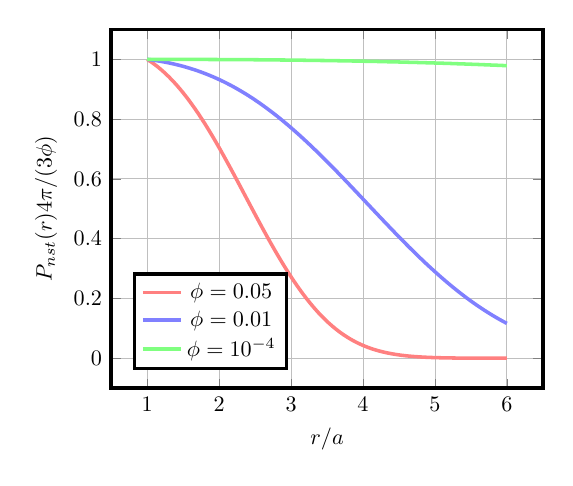
\begin{tikzpicture}[scale=0.8]
    \begin{axis}[
        xlabel={$r/a$},
        ylabel={$P_\text{nst}(r) 4\pi/ (3\phi) $},
        legend style={at={(0.05,0.05)}, anchor=south west},
        grid=major,
        domain=1:6,
        samples=100,
        ultra thick
    ]
    
    % Plot for phi = 0.05
    \addplot[color=red!50,ultra thick]
    { exp(-0.05 * (x^3 - 1))};
    \addlegendentry{$\phi = 0.05$}
    
    % Plot for phi = 0.01
    \addplot[color=blue!50,ultra thick]
    { exp(-0.01 * (x^3 - 1))};
    \addlegendentry{$\phi = 0.01$}
    
    % Plot for phi = 0.001
    \addplot[color=green!50,ultra thick]
    { exp(-0.0001 * (x^3 - 1))};
    \addlegendentry{$\phi = 10^{-4}$}
    
    \end{axis}
\end{tikzpicture}
\hfil
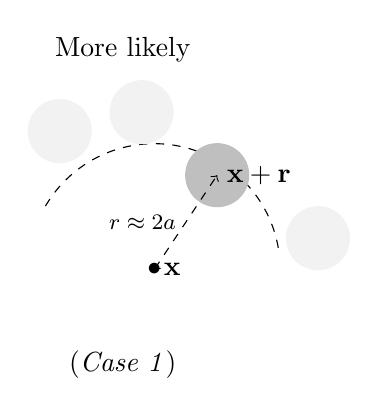
\begin{tikzpicture}[scale=0.8]
  \filldraw[ gray!10!white](+2.6,0.5)circle (0.5);
  \filldraw[ gray!10!white](-1.5,2.2)circle (0.5);
  \draw[dashed](10:2) arc (10:150:2);
  % \filldraw[ gray!50!white](0,0) circle (0.5);
  \filldraw[ gray!50!white](1,1.5)circle (0.5);
  \filldraw[ gray!10!white](-0.2,2.5)circle (0.5);
  \draw(0,0)node{$\bullet$}node[right]{$\textbf{x}$};
  \draw[dashed,<->](0,0)--(1,1.5)node[midway,left]{\footnotesize $r\approx 2 a$}node[right]{$\textbf{x}+\textbf{r}$};
  % \draw[dashed](-0.2,3.5);
  \node[ultra thick] (title) at (-0.5,3.5) {{More likely}};
  \node[ultra thick] (title) at (-0.5,-1.5) {(\textit{Case 1})};
\end{tikzpicture} 
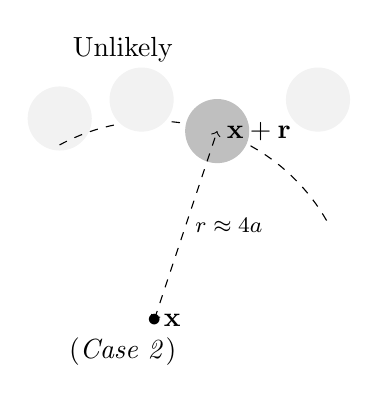
\begin{tikzpicture}[scale=0.8]
  \filldraw[ gray!10!white](+2.6,3.5)circle (0.5);
  \filldraw[ gray!10!white](-1.5,3.2)circle (0.5);
  \draw[dashed](30:3.16) arc (30:120:3.16);
  % \filldraw[ gray!50!white](0,0) circle (0.5);
  \filldraw[ gray!50!white](1,3)circle (0.5);
  \filldraw[ gray!10!white](-0.2,3.5)circle (0.5);
  \draw(0,0)node{$\bullet$}node[right]{$\textbf{x}$};
  \draw[dashed,<->](0,0)--(1,3)node[midway,right]{\footnotesize  $r\approx 4a$}node[right]{$\textbf{x}+\textbf{r}$};
  % \draw[dashed](-0.2,3.5);
  \node[ultra thick] (title) at (-0.5,4.3) {{Unlikely}};
  \node[ultra thick] (title) at (-0.5,-0.5) {(\textit{Case 2})};
\end{tikzpicture} 
\caption{(left) Plot of the normalized nearest neighbor distribution $P_\text{nst}$. 
(right) Sketches explaining the behavior of the nearest neighbor distribution $P_\text{nst}$: 
(\textit{Case 1}) A droplet located at $\textbf{x}+\textbf{r}$ relatively \underline{close} to a point occupied by the continuous phase at \textbf{x}; this situation is likely to happen. 
(\textit{Case 2}) A droplet located at $\textbf{x}+\textbf{r}$ relatively \underline{far} to a point occupied by the continuous phase at \textbf{x}; this situation very unlikely to happen.
Indeed, it implies that no particles are present within the sphere of radius $4a$ centered at $\textbf{x}$ since the nearest neighbor is located at a distance $4a$. 
}
\label{fig:P_nst_f}
\end{figure}
With these assumptions in place, we can compute the \textit{Reynolds stress} using, \ref{eq:relation_ensemble_nst} which reduces to the following formula, 
\begin{equation}
    \avg{\chi_f \textbf{u}_f'\textbf{u}_f'}
    = 
    \frac{3\phi}{4\pi}
    \int_{\mathbb{R}^6}
    \textbf{v}_f^\text{nst}
    \textbf{v}_f^\text{nst}
     e^{-\phi(r^3 -1)}
    d\textbf{r}
    d\textbf{w},
    \label{eq:step_one}
\end{equation}
where it must be understood that $\textbf{v}_f^\text{nst}$ is given by \ref{eq:stokes_sol}. 


Before computing the integration for Stokes flows we would like to apply this formulation to re-compute the \textit{Reynolds stress} of translating bubbles in potential flows. 
Indeed, it can be show that \ref{eq:solution_isolated_at_x} also hols for the \textit{nearest neighbor conditionally averaged} momentum equations in potential flows, thus in that case $\textbf{v}^\text{nst}_f \approx \textbf{u}_f^{1d}$ where we recall that $ \textbf{u}_f^{1d}$ is given by \ref{eq:potential_sol}
Therefore, we carry out the direct integration of \ref{eq:step_one} using \ref{eq:potential_sol} and obtain, 
\begin{equation}
    \avg{\chi_f \textbf{u}_f'\textbf{u}_f'}
    = \Gamma_\text{inc}(-1,\phi)\phi^2 e^\phi \left\{
        \frac{1}{20}[\textbf{u}_{fp}\textbf{u}_{fp}+ \frac{1}{n_p}\pavg{\textbf{u}_\alpha\textbf{u}_\alpha}]
        + 
        \frac{3}{20} (\textbf{u}_{fp}\cdot \textbf{u}_{fp} + 2k_p)\bm\delta
    \right\},
    \label{eq:potential_nst}
\end{equation}
where $\Gamma_\text{inc}$ is the gamma incomplete function. 
According to \ref{eq:potential_nst} our results differ with \ref{eq:van_wingarden_sol} by a factor of $\Gamma_\text{inc}(-1,\phi)\phi^2 e^\phi$. 
Nevertheless, this inconsistency is easily solved noticing that $\Gamma_\text{inc}(-1,\phi)\phi^2 e^\phi \sim \phi + \mathcal{O}(\phi^2)$. 
Thus, we conclude that at the leading order, our methodology seem consistent with the classical conditional average methodology introduced by \citet{batchelor1972sedimentation}. 

Now that we have all the tools in hand, let us carry out the direct integration of \ref{eq:step_one} for the wake of a spherical droplet in stokes flows. 
Indeed, using \ref{eq:solution_isolated_at_x} and \ref{eq:Pnst_explicit} in \ref{eq:step_one} gives, in dimensionless form,  
\begin{equation}
    \avg{\chi_f  \textbf{u}_f'\textbf{u}_f'}^*
    = \phi    
    C_1
    \left\{
        \textbf{u}_{fp}\textbf{u}_{fp}+ \frac{1}{n_p}\pavg{\textbf{u}_\alpha'\textbf{u}_\alpha'}
        -\frac{1}{3} (\textbf{u}_{fp}\cdot \textbf{u}_{fp} + 2k_p)\bm\delta
    \right\},    
    + \phi C_2
    (\textbf{u}_{fp}\cdot \textbf{u}_{fp} + 2k_p)\bm\delta,
    \label{eq:final_closure}
\end{equation}
with,
\begin{align*}
    C_1(\phi,\lambda)
    = \frac{1}{20(1+l)^2}\left[
        \frac{9(2+3\lambda)^2}{4}\Gamma(1/3) \phi^{-1/3}
        - (27+82\lambda +62\lambda^2)
    \right],\\
    C_2(\phi,\lambda)
    = \frac{1}{6(1+l)^2}\left[
        \frac{(2+3\lambda)^2}{4}\Gamma(1/3) \phi^{-1/3}
        - (3+10\lambda +8\lambda^2)
    \right].
\end{align*}
\tb{maybe remove order phi terms}
We have decomposed the \textit{Reynolds stress} tensor into two contribution. 
The first one being, a traceless symmetric tensor, proportional to the functional $C_1$. 
The second contribution is the isotropic part of the \textit{Reynolds stress} tensor, which is proportional to $C_2$. 
This result deserves some comments. 

Firstly, we can notice that, according to the value of $C_1$ and $C_2$, the \textit{pseudo turbulence} or \textit{Reynolds stress} induced by the translation of the droplets is higher for large values of $\lambda$. 
In other words the solid particle induce more wake than a bubble of the same size. 

Secondly, as witnessed by the presence of the term $\phi^{-1/3}$, in $C_1$ and $C_2$, we conclude that the solution obtained here is still consistent with the observation made in \ref{eq:real_error} or in \citet{caflisch1985variance}. 
Indeed, for an isolated droplet, i.e. when we take the limit, $\phi \to 0$, we obtain $\lim_{\phi \to 0} \avg{\chi_f \textbf{u}_f' \textbf{u}_f'} / \phi = \infty$. 
Consequently, in agreement with the previous statements, the normalized \textit{Reynolds stress} is infinite for an isolated droplet, however when considering small but finite value of $\phi$ the \textit{Reynolds stress} remains finite and is given by \ref{eq:final_closure}. 

Finally, as it is not the \textit{Reynolds stress} divided by $\phi$ that matter, but $\avg{\chi_f\textbf{u}_f'\textbf{u}_f'}$ it self, notice that at the leading order in $\phi$ we obtain,  $\avg{\chi_f\textbf{u}_f'\textbf{u}_f'}\sim\phi^{2/3}$. 
Notably, this  trend in $\sim\phi^{2/3}$ is not new and agree with previous studies found in the literature.
Specifically, in \citet{hill2001first} they compute \textit{Reynolds stress} for ordered array of spheres and found $k_f \sim 0.969 \phi^{2/3}$. 
This nearly agree with our \ref{eq:final_closure} with $\lambda =\infty$ as it gives, $k_f  = 1.50$. 



\subsection{The solution at higher order. }

Although we chose to neglect the source term in \ref{eq:momentum_nst_d_stokes} how can we be certain that it was indeed negligible ? 
Even though this term is $\mathcal{O}(\phi)$ higher than the others in $\textbf{v}^\text{nst}$, it does not necessarily imply that it will contribute at $\mathcal{O}(\phi)$ higher than the other terms in $\avg{\rho_f\chi_f \textbf{u}_f'\textbf{u}_f'}$. 
Indeed, in \citet{zhang2021ensemble}, while carrying similar derivation foundout that the terms of $\mathcal{O}(\phi)$ in $\textbf{v}^\text{nst}$ contributed to $\mathcal{O}(\phi^{1/3})$ in their final results. 
In other worlds, this is not as straightforward as in the \textit{single-particles conditional averaged} equations. 

\subsubsection{The velocity fields singularity solution}

Regardless of the right-hand side of \ref{eq:momentum_nst_d_stokes} the boundary condition at the surface of the particle, located at \textbf{y}, will generate the velocity fields\citep{pozrikidis1992boundary}, 
\begin{equation}
    \textbf{v}^\text{nst}_p[\textbf{z},t|\textbf{x},\textbf{w},\textbf{y}]
    = 
    \frac{a}{4}(\textbf{w}- \textbf{u}[\textbf{y},t])\cdot\left[
        \frac{2+3\lambda}{1+\lambda}
        +
        a^2\frac{\lambda}{2(1+\lambda)}\pddz^2 
    \right]\mathcal{G}(\textbf{z},\textbf{y}).
    \label{eq:solution_isolated2}
\end{equation}
Where $\mathcal{G}(\textbf{z},\textbf{y})$ is still the Ossen tensor, or Green function of the stokes equations. 
\tb{En principe la vitesse relative est forme avec la bulk velocity }

Now let us turn our attention to the source term on the right-hand side of \ref{eq:momentum_nst_d_stokes}. 
Following \citet{zhang2021ensemble}, we remark that the contribution to the velocity field, generated by the particle free zone, can be written as a sum of \textit{Stokeslets} of magnitude $\phi\Delta \rho |\textbf{g}|$.
Indeed, the velocity field evaluated at \textbf{z} generated by the point force:  $\phi\Delta \rho \textbf{g}$, located at a generic point $\textbf{x}'$, can be written \citep{pozrikidis1992boundary}, 
\begin{equation}
    \frac{\phi\Delta \rho \textbf{g}}{8\pi \mu_f}\cdot \mathcal{G}(\textbf{z},\textbf{x}')
\end{equation}
Consequently, the velocity fields generated by the particle-free zone, as given in \ref{fig:unst}, can be written \citep{zhang2021ensemble}, 
\begin{equation}
    \textbf{v}_b^\text{nst}[\textbf{z},t|\textbf{y},\textbf{w},\textbf{x}]
    = 
    \frac{\phi\Delta \rho \textbf{g}}{8\pi \mu_f}\cdot 
    \int_{|\textbf{x}'-\textbf{x}|< |\textbf{y}- \textbf{x}|}
    \mathcal{G}(\textbf{z},\textbf{x}')
    d\textbf{x}'
    \label{eq:v_b_sol}
\end{equation}
where we used the subscript $_b$ to denote the particle free zone contribution. 
Due to the linearity of the Stokes equations, the total velocity field is thus the sum of \ref{eq:solution_isolated2} and \ref{eq:v_b_sol}. 
% Likewise, the stress generated by the particle free-zone might be written \citep{pozrikidis1992boundary},
% \begin{equation}
%     \bm\sigma_b^\text{nst}[\textbf{z},t|\textbf{y},\textbf{w},\textbf{x}]
%     = 
%     \frac{\phi\Delta \rho \textbf{g}}{8\pi}\cdot 
%     \int_{|\textbf{x}'-\textbf{x}|< |\textbf{y}- \textbf{x}|}
%     \mathcal{T}(\textbf{z},\textbf{x}')
%     d\textbf{x}'
%     \label{eq:sigma_b_sol}
% \end{equation}
% with, 
% \begin{equation}
%     \mathcal{T}(\textbf{z},\textbf{x}')
%     = - 6\frac{\textbf{rrr}}{r^5}. 
% \end{equation}
% Here, $\textbf{r} = \textbf{z} - \textbf{x}'$. 

Therefore, the total velocity field $\textbf{v}^\text{nst}_f$ at the point $\textbf{x}$, can be obtained using \ref{eq:v_b_sol} and \ref{eq:solution_isolated2} evaluated at the point \textbf{x}, and  \ref{eq:reformulation}, which yields,  
\begin{multline}
    \textbf{v}^\text{nst}_f [\textbf{x},\textbf{w},\textbf{y},t]
    =
    \frac{a}{4}(\textbf{w}- \textbf{u}[\textbf{y},t])\cdot\left[
        \frac{2+3\lambda}{1+\lambda}
        +
        a^2\frac{\lambda}{2(1+\lambda)}\grad^2 
    \right]\mathcal{G}(\textbf{x},\textbf{y})\\
    +
    \phi(\textbf{u}_d - \textbf{u}_f)
    + 
    \frac{\phi\Delta \rho \textbf{g}}{8\pi \mu_f}\cdot 
    \int_{|\textbf{x}'-\textbf{x}|< |\textbf{y}- \textbf{x}|}
    \mathcal{G}(\textbf{x},\textbf{x}')
    d\textbf{x}',
\end{multline}
Carrying out the integral on the second line gives directly,
\begin{equation}
    \int_{|\textbf{x}'-\textbf{x}|< |\textbf{y}- \textbf{x}|}
    \mathcal{G}(\textbf{x},\textbf{x}')
    d\textbf{x}'
    = \frac{8\pi}{3}|\textbf{x}- \textbf{y}|^2\bm\delta
\end{equation}
which finally gives the result, 
\begin{multline}
    \textbf{v}^\text{nst}_f
    =
    \frac{a}{4}(\textbf{w}- \textbf{u}[\textbf{y},t])\cdot\left[
        \frac{2+3\lambda}{1+\lambda}
        +
        a^2\frac{\lambda}{2(1+\lambda)}\grad^2 
    \right]\mathcal{G}(\textbf{x},\textbf{y})
    + 
    \frac{\phi\Delta \rho \textbf{g}}{3\mu_f} |\textbf{x}-\textbf{y}|^2
    +
    \phi(\textbf{u}_d - \textbf{u}_f)
    \label{eq:final_sol_v_nst}
\end{multline}
In this expression we clearly identify $3$ distinct contributions. 
Indeed, the first two terms on the right-hand side of \ref{eq:final_sol_v_nst} correspond to the disturbance field generated by an isolated droplet, which was the only contribution in \ref{eq:solution_isolated_at_x}. 
The third term corresponds to the ``back flow velocity'' as called by \citet{zhang2021ensemble}, it refers to the flow generated by the particle-free zone. 
Finally, the last term ensure that we stay in the right reference frame. 
Notice that in \citet[Appendix A]{zhang2021ensemble} they carried out nearly the same calculation for solid particles.
Apart from that, one can note a small differences between \ref{eq:final_sol_v_nst} with $\lambda = \infty$ and his Equation (B 4), indeed, while we have got$(\textbf{w}- \textbf{u}_f[\textbf{y},t])$ as factor of the first term, he obtained $(\textbf{w}- \textbf{u}_f - \textbf{v}_b^\text{nst})$. 
This is due to the different reference frame used for the velocity fields, indeed, while we have got only one source term at the right-hand side of \ref{eq:momentum_nst_d_stokes} he has a supplementary, constant source term. 
This is the reason for the presence of his $\textbf{v}_b'$ which is not in \ref{eq:final_sol_v_nst}. 
Thus, everything is well consistent, Additionally we generalized and demonstrated his results for droplets. 


For a better physical understanding we present know the dimensionless form of \ref{eq:final_sol_v_nst}. 
The lengths are made dimensionless using the radius of the particle $a$, the velocity vector $\textbf{w} - \textbf{u}$ is made dimensionless the norm $U = |\textbf{w} - \textbf{u}_f|$, 
Indeed, we have the relation, 
\begin{equation*}
    \frac{\textbf{w} - \textbf{u}}{|\textbf{w} - \textbf{u}_f|}
    = \textbf{e} + \phi \textbf{e}
\end{equation*}
where we introduced the unit vector: $\textbf{e} = \textbf{w} - \textbf{u}_f/U$. 
Likewise, the gravity acceleration vector is made dimensionless using its norm, such that the unit vector in the direction of the acceleration of gravity is given by $\textbf{k} = \textbf{g} / g$, with $g = |\textbf{g}|$. 
Dividing \ref{eq:final_sol_v_nst} by $U$ and using these definitions yields directly the dimensionless expression for the disturbance velocity field, 
\begin{equation}
    \frac{\textbf{v}^\text{nst}_f}{U}
    =
    \frac{1}{4}(\textbf{e}+ \phi \textbf{e})\cdot\left[
        \frac{2+3\lambda}{1+\lambda}
        +
        \frac{\lambda}{2(1+\lambda)}\grad^2 
    \right]\mathcal{G}(\textbf{x},\textbf{y})
    + \phi A |\textbf{x}-\textbf{y}|^2 \textbf{k}
    +\phi \textbf{e}
    \label{eq:v_nst_solution_adim}
\end{equation}
\tb{The $(\textbf{e}+ \phi \textbf{e})$ shoud either be remove or re-dim }
where we kept the same notation for all the distances, they are assumed implicitly dimensionless. 
At the leading order, notice that the terms proportional to $\phi \textbf{e}$ in \ref{eq:v_nst_solution_adim} are negligible, however we keep them for the purpose of generality. 
Additionally, we introduced the dimensionless number, 
\begin{equation}
    A = \frac{Ar}{12 Re}=\frac{\Delta \rho g (2a)^2}{12 \mu_f U}
    \label{eq:A_general}
\end{equation}
where we recall that $Ar$ is the \textit{Galileo} number and $Re$ the \textit{Reynolds} number, defined as,  
\begin{align*}
    Re= \frac{\rho_f U 2a}{\mu_f},
    &&
    Ar = \frac{\rho_f \Delta\rho g (2a)^3}{\mu_f^2},
\end{align*}
respectively. 
Upon considering specific scenarios, such as a steady state rising droplet due to the acceleration of gravity, one is able to relate $Ge$ and $Re$ and give explicit closure instead of $A$. 
As mentionned in \citet{zhang2021ensemble} this approaches can be generalized to other body forces fields, such as electromagnetic forces, in order to obtain the influence of the latter on the resulting velocity field.

\subsubsection{The pseudo turbulent tensor closure}

From \ref{eq:sol_dimenisonless_results} we may already compute the integral in \ref{eq:step_one}. 
However, as $\textbf{e}$ and $\textbf{k}$ in \ref{eq:sol_dimenisonless_results}  are not necessarily collinear vectors the functional form of the resulting stress tensor is not trivial. 
% Thus, in the first place we clarify the expected functional form of $\avg{\rho_f \textbf{u}_f'\textbf{u}_f'}$. 
Indeed, since $\textbf{v}_f^\text{nst}\sim \textbf{e}$ or $\textbf{g}$, the final results must be a tensor built from sum of product of these two vectors.  
Additionally, since $\avg{\rho_f \textbf{u}_f'\textbf{u}_f'}$ is a symmetric tensor, the result must be a symmetric tensor as well. 
Since, the only second order symmetric tensors that can be constructed from the  two arbitrary vectors: $\textbf{e}$ and $\textbf{k}$ are, 
\begin{align*}
    \textbf{ee}
    && (\textbf{e}\cdot \textbf{e})\bm\delta, 
    && \textbf{kk},
    && (\textbf{k}\cdot \textbf{k})\bm\delta,
    && \textbf{ke}+\textbf{ek},
    && (\textbf{k}\cdot \textbf{e})\bm\delta, 
\end{align*}
we deduce that the volume integral of \ref{eq:step_one}, have the form, 
\begin{align}
    \frac{1}{U^2}
    \frac{3\phi}{4\pi}\int_{\mathbb{R}^3}
    \textbf{v}_f^\text{nst}
    \textbf{v}_f^\text{nst}
     e^{-\phi(r^3 -1)}
    d\textbf{r}
    &= C^{(1)}_e \left[
        \textbf{ee}
         - \frac{1}{3}(\textbf{e}\cdot \textbf{e})\bm\delta
    \right]
    + C^{(2)}_e 
    (\textbf{e}\cdot \textbf{e})\bm\delta \nonumber \\
    &+ C^{(1)}_k \left[
        \textbf{kk}
         - \frac{1}{3}(\textbf{k}\cdot \textbf{k})\bm\delta
    \right]
    + C^{(2)}_k 
    (\textbf{k}\cdot \textbf{k})\bm\delta \nonumber \\
    &+ C^{(1)}_{ek} \frac{1}{2}\left[
        (\textbf{ek}  + \textbf{ke})
         - \frac{2}{3}(\textbf{k}\cdot \textbf{e})\bm\delta
    \right]
    + C^{(2)}_{ek} 
    (\textbf{e}\cdot \textbf{k})\bm\delta 
    \label{eq:functional_form}
\end{align}
where the first term of each line correspond to symmetric traceless tensors, and the second term of each line to the corresponding isotropic contribution. 
Then, the first two constant, $C^{(1)}_e$ and $C^{(2)}_e$ can be obtained setting $\textbf{g}= 0$ in \ref{eq:sol_dimenisonless_results} and performing the integration. 
Likewise, $C^{(1)}_k$ and $C^{(2)}_k$ can be obtained setting $\textbf{e}=0$ in \ref{eq:sol_dimenisonless_results}. 
The constants, $C^{(1)}_{ek}$ and $C^{(2)}_{ek}$ can be obtained setting $\textbf{g} = 0$ in of the $\textbf{v}_f^\text{nst}$ on the left-hand side of \ref{eq:functional_form} and $\textbf{e}=0$ in the other $\textbf{v}_f^\text{nst}$. 
Thus, we directly, obtain at the leading order, 
\begin{align}
    C_e^{(1)} =
    % \frac{9(2+3\lambda)^2 \Gamma(\frac{1}{3})}{80(\lambda+1)^2}\phi^{2/3}
    \frac{27}{10}
    C_e^{(2)}
    % + \mathcal{O}(\phi)
    &&  C_e^{(2)} =
    \frac{(2+3\lambda)^2 \Gamma(\frac{1}{3})}{24(\lambda+1)^2}\phi^{2/3}
    + \mathcal{O}(\phi)
    \\
    C_k^{(1)} =
    % A^2 \Gamma\left(7/3\right)\phi^{2/3}
    3
    C_k^{(2)}
    % + \mathcal{O}(\phi^{5/3})
    && C_k^{(2)} =
    A^2 \frac{\Gamma(\frac{7}{3})}{3}\phi^{2/3}
    + \mathcal{O}(\phi^{5/3})
    \\
    C_{eg}^{(1)} =
    3
    C_{eg}^{(2)}
    % A\frac{2 (2+3\lambda) \Gamma(\frac{4}{3})}{3 (\lambda+1)}\phi^{2/3}
    % + \mathcal{O}(\phi^{4/3})
    && C_{eg}^{(2)} =
    A\frac{2 (2+3\lambda) \Gamma(\frac{4}{3})}{9(\lambda+1)}\phi^{2/3}
    + \mathcal{O}(\phi^{4/3})
    \label{eq:constants}
\end{align}
As can be seen, the leading order contribution from the back flow velocity generated due to the acceleration of gravity is $\sim \phi^{2/3}$. 
It is therefore non-negligible in this general framework. 
\tb{include the orer phi terms .  ?  ? ? }


Following \ref{eq:step_one} to obtain the \textit{Reynolds stress} tensor we now integrate  \ref{eq:functional_form} over the $\textbf{w}$, which yield the final form of our \textit{Pseudo turbulent} tensor model, namely, 
\begin{align}
    \frac{\avg{\chi_f \textbf{u}_f'\textbf{u}_f'}}{U^2}
    &= 
    C^{(1)}_e \left[
        \textbf{e}_p\textbf{e}_p
        + \frac{\pavg{\textbf{u}_\alpha'\textbf{u}_\alpha'}}{n_p U^2}
         - \frac{1}{3}(\textbf{e}_p\cdot \textbf{e}_p+2k_p/U^2)\bm\delta
    \right]
    + C^{(2)}_e 
    (\textbf{e}_p\cdot \textbf{e}_p+2k_p/U^2)\bm\delta \nonumber \\
    &+ C^{(1)}_k  \left[
        \textbf{kk}
         - \frac{1}{3}(\textbf{k}\cdot \textbf{k})\bm\delta
    \right]
    +C^{(2)}_k 
    (\textbf{k}\cdot \textbf{k})\bm\delta \nonumber \\
    &+ C^{(1)}_{ek} \left[
        \frac{1}{2}
        (\textbf{e}_p\textbf{k}  + \textbf{k} \textbf{e}_p)
         - \frac{1}{3}(\textbf{k}\cdot \textbf{e}_p)\bm\delta
    \right]
    + C^{(2)}_{ek}
    (\textbf{e}_p\cdot \textbf{k})\bm\delta 
    \label{eq:functional_form_avg}
\end{align}
In this expression $\textbf{e}_p = \int \textbf{e} d\textbf{w} $ represents the mean direction of the mean relative phase velocity $\textbf{u}_{pf}$ such that $\textbf{u}_{pf} = U \textbf{e}_p$, in opposition to $\textbf{e}$ which represented the direction of a single particle relative velocity. 



In summary, the only additional terms appearing due to the integration over the velocity phase space is the addition of the particle fluctuation contribution to the \textit{Reynolds stress}. 
However, it is likely that $k_p/U^2 \sim \phi$ at least, therefore at $\mathcal{O}(\phi)$ this term might be safely neglected. 
However, for purpose of generality we keep these terms. 



\subsubsection{Steady-state rising droplet}

Let us now study the case where $\textbf{k} = - \textbf{e} = \textbf{e}_z$, meaning that the droplet rises in the opposite direction of gravity which is aligned with the vertical direction denoted by $\textbf{e}_z$.  
At $\mathcal{O}(\phi)$ and in Stokes flow regime, the drag applied on an isolated spherical droplet is given by Hadamard-Ribczynski formula, thus at steady-state the rising velocity of a droplet is given by, 
\begin{equation}
    U = \Delta \rho \frac{g (2a)^2}{6 \mu_f }\left(\frac{1+\lambda}{2+3\lambda}\right).
    \label{eq:U_isolated}
\end{equation}
% \begin{equation}
%     2a \pi \mu_f \left(\frac{3\lambda +2}{\lambda +1}\right) 
%     U
%     = 
%     \frac{4}{3}\pi a^3 
%     \Delta \rho
%     g,
% \end{equation}
We deduce from this relation that in this specific situation, i.e. when the direction of the relative velocity \textbf{e} is aligned with the gravity acceleration direction, we have, 
\begin{equation}
    A = \frac{1}{2}\left(\frac{3\lambda +2}{\lambda +1}\right). 
    \label{eq:closure_A}
\end{equation}
Injecting this expression into \ref{eq:v_nst_solution_adim} gives us an explicit expression of the velocity field $\textbf{v}^\text{nst}_f$. 

To give a better idea of the meaning of $\textbf{v}_f^\text{nst}$, we display 
in \ref{vnst_vertical} the streamlines generated by the field $\textbf{v}_f^\text{nst}(\textbf{r})$ in the cross-section, given by the plane formed by the vectors $(\textbf{e}_x,\textbf{e}_z)$. 
\begin{figure}[h!]
    \centering
    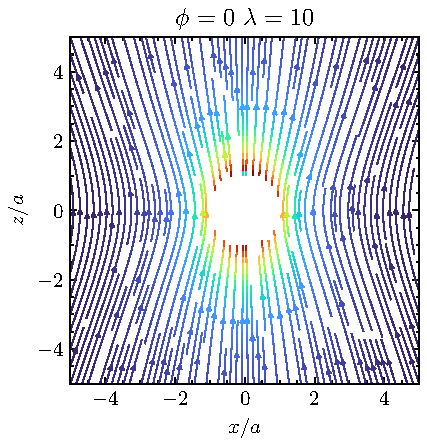
\includegraphics[height = 0.33\textwidth]{image/Vnst_l_10_0.pdf}
    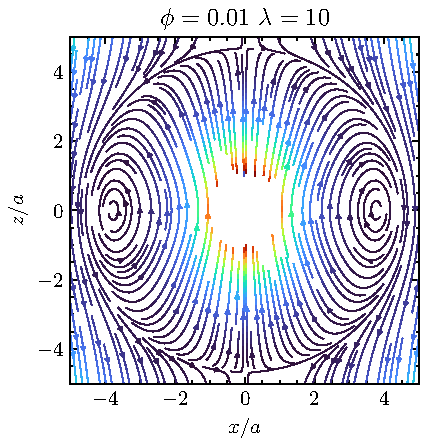
\includegraphics[height = 0.33\textwidth]{image/Vnst_l_10_1.pdf}
    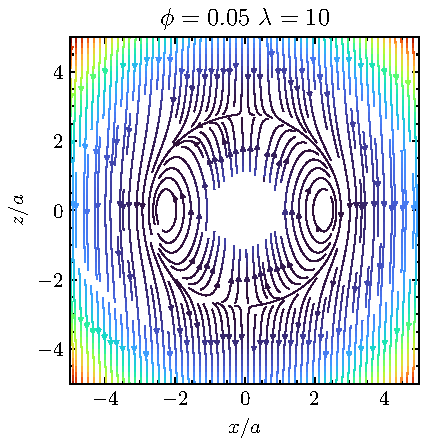
\includegraphics[height = 0.33\textwidth]{image/Vnst_l_10_5.pdf}
    % 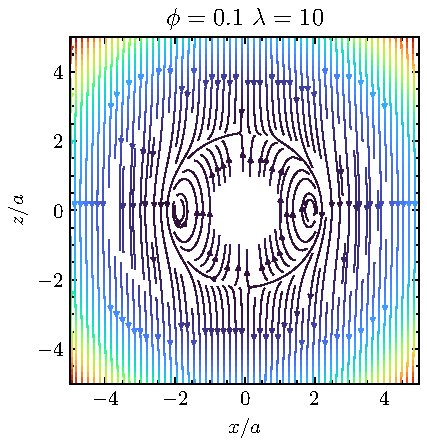
\includegraphics[height = 0.33\textwidth]{image/Vnst_l_10_10.pdf}
    \caption{Streamlines of the disturbance velocity field $\textbf{v}^\text{nst}(\textbf{r}_f)$ \eqref{eq:v_nst_solution_adim}  in the cross-section given by the plane $(\textbf{e}_x,\textbf{e}_z)$, for multiples volume fraction $\phi = 0, 0.01$ and $0.05$ at $\lambda = 10$.  
    The color map indicates the magnitude of the velocity, from black which corresponds to a velocity magnitude of 0, to the color at the interface which corresponds to 1.
    In this situation $\textbf{e} = \textbf{e}_z$ and $\textbf{k} = -\textbf{e}_z$}
    \label{fig:vnst_vertical}
\end{figure}
We can observe on \ref{fig:vnst_vertical} (left) that $\textbf{v}^\text{nst}_f(\phi =0)$ corresponds to the disturbance field of an isolated particle in Stokes flow. 
This is easily understandable considering that the last two terms on the right-hand side of \ref{eq:v_nst_solution_adim} cancel for $\phi=0$, thus leading to \ref{eq:solution_isolated} which is the solution for isolated particle. 
At finite volume fraction, $\phi =0.01$, we  observe in \ref{fig:vnst_vertical} (middle), that a downstream velocity start to appear at large distance from the particle center.  
As discussed previously, this ``back flow velocity'' is given by the term $\phi A |\textbf{x}- \textbf{y}|^2 \textbf{k}$ in \ref{eq:solution_isolated}.
The particle is thus surrounded by a spherical shell within which the disturbance field has a positive vertical velocity, and outside which the velocity is negative.
In the following discussion we call this spherical shell the \textit{confinement zone}.   
For higher volume fractions $\phi = 0.05$, the backflow velocity is even stronger leading to a smaller confinement zone around the particle. 

Let us discuss the form of \ref{eq:functional_form_avg} in the specific case displayed in \ref{fig:vnst_vertical}, i.e. spherical droplets rising in stokes flow. 
Since $\textbf{e}_p = - \textbf{k}$ we have $\textbf{e}_p\textbf{k} = - \textbf{kk}$. 
Additionally, one can use \ref{eq:closure_A} into the expression for $C_k^{(1)}$ and $C_{ek}^{(1)}$. 
In this specific case, by carrying out the calculation, we obtain, 
\begin{equation}
    C_k^{(1)} \textbf{kk} + C_{ek}^{(1)} \textbf{ke}_p
    = 0. 
    \label{eq:cancelation1}
\end{equation}
Applying the same reasoning, one can also deduce that, 
\begin{equation}
    C_k^{(2)} \textbf{k}\cdot \textbf{k} + C_{ek}^{(2)} \textbf{k}\cdot \textbf{e}_p
    = 0. 
    \label{eq:cancelation2}
\end{equation}
Consequently, we must deduce that the contribution from the gravity acceleration to the \textit{Reynolds stress} tensor, remains negligible in this simplified situation. 
This, might seem surprising considering the seemingly non-negligible action of the gravity on the velocity field displayed \ref{eq:vnst_vertical}. 
However, we must understand from this fact, that the velocity variance generated by the back flow velocity, also induce a decrease of the velocity variance generated by the particle motion compared to the isolated case.
In other word, the back flow velocity generate at the boundaries of the confinement zone a low velocity variance, which is exactly balanced by the velocity variance generated by the back flow at the exterior of the confinement zone.    
Notice that this explanation is only true when, $\textbf{k} = - \textbf{e}_p$. 
Thus, we may examine now situations were the velocity of the dispersed phase is not in the opposite direction of gravity. 



\subsubsection{Horizontal motions}

We now consider the case were $\textbf{e}_p = \textbf{e}_x$, and $\textbf{k} = - \textbf{e}_z$, where $\textbf{e}_z$ is still the vertical unit vector and $\textbf{e}_x$ the Horizontal unit vector. 
Of course in the steady-state isolated regime $\textbf{e}_p$, could not be otherwise than vertical. 
However, in a more general case, consider an Euler-Euler framework for example, $\textbf{e}_p$ have absolutely no reason to be in the vertical direction, due to boundaries or transient effects. 
In this case $A$ is given by \ref{eq:A_general} and requires the norm of the relative velocity $U$ which is supposed known in the Euler-Euler simulation. 

\begin{figure}[h!]
    \centering
    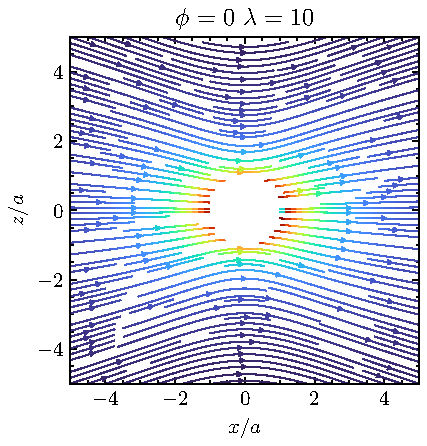
\includegraphics[height = 0.33\textwidth]{image/Vnst_H_l_10_0.pdf}
    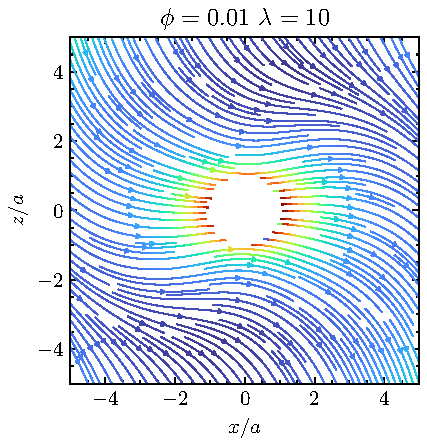
\includegraphics[height = 0.33\textwidth]{image/Vnst_H_l_10_1.pdf}
    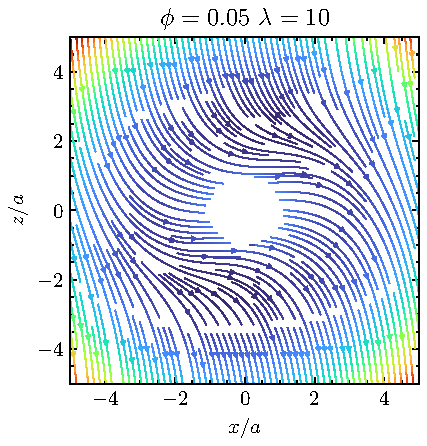
\includegraphics[height = 0.33\textwidth]{image/Vnst_H_l_10_5.pdf}
    % 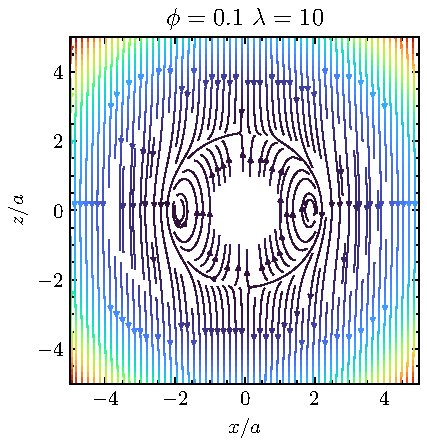
\includegraphics[height = 0.33\textwidth]{image/Vnst_l_10_10.pdf}
    \caption{Streamlines of the disturbance velocity field $\textbf{v}^\text{nst}(\textbf{r}_f)$  \eqref{eq:v_nst_solution_adim} in the cross-section given by the plane $(\textbf{e}_x,\textbf{e}_z)$, for multiples volume fraction $\phi = 0, 0.01$ and $0.05$ at $\lambda = 10$.  
    The color map indicates the magnitude of the velocity, from black which corresponds to a velocity magnitude of 0, to the color at the interface which corresponds to 1.
    In this situation $\textbf{e} = \textbf{e}_x$ and $\textbf{k} = -\textbf{e}_z$.
    The constant $A$ have been arbitrarily set to $1$. }
    \label{fig:vnst_horizontal}
\end{figure}
In \ref{fig:vnst_horizontal} we display the streamlines generated by the velocity field $\textbf{v}_f^\text{nst}$ in this situation. 
As before, we remark that at $\phi = 0$, $\textbf{v}_f^\text{nst}$ corresponds to the disturbance velocity field of an isolated droplet translating Horizontally in Stokes flow. 
At $\phi = 0.01$, see \ref{fig:vnst_horizontal} (middle), the effect of gravity induce a downstream flow, which is, this time not in the opposite direction of the disturbance velocity of the drop, resulting into a global down-right flow. 
At higher volume fraction this down stream flow is stronger, and the confinement zone around the particle smaller. 
In summary, we observe the same phenomenon as in the previous situation reported on \ref{fig:vnst_vertical}, except that the droplet disturbance field is not in the opposite direction of the back flow velocity, but normal to it.

This difference has a significant impact on the \textit{Reynolds stress} closure, as the relation \ref{eq:cancelation1} and \ref{eq:cancelation2} are not true anymore. 
Indeed, in this case the functional form of the \textit{Reynolds stress} is given by, 
\begin{equation}
    \frac{\avg{\chi_f \textbf{u}_f'\textbf{u}_f'}}{U^2}
    = 
    C^{(1)}_e 
    \textbf{e}_x\textbf{e}_x
    % + \frac{\pavg{\textbf{u}_\alpha'\textbf{u}_\alpha'}}{n_p U^2}
    +C^{(1)}_k    
    \textbf{e}_z\textbf{e}_z
    - C^{(1)}_{ek} 
        \frac{1}{2}
        (\textbf{e}_x\textbf{e}_z+ \textbf{e}_z \textbf{e}_x)
    + [C^{(2)}_e + C^{(2)}_k - (C^{(1)}_k + C^{(1)}_e )/3 ]  \bm\delta. 
\end{equation}
Thus, the contribution from the wake of the particles is still present and given by $C_e^{(1)}$ and $C_e^{(2)}$. 
Regarding the buoyancy forces, it provides additional contributions that are on the vertical direction. 
Finally, the cross term $\textbf{e}_p \textbf{k}$ provides off-diagonal terms. 
The isotropic part of this tensor is the sum of the aforementioned contributions. 

\subsection{Discussion}

In this section we have considered the translating motion of a spherical droplet in stokes flow. 
In this regime we have shown that the ambient body force field $\textbf{g}$ plays a non-negligible role on the \textit{Nearest Neighbor Conditional Averaged} disturbance fields. 
Consequently, the \textit{Reynolds stress} closure obtained is a function of $\textbf{u}_{fp}$ the relative phase velocity and the direction of $\textbf{g}$ which is considered vertical. 

To extend this model one might consider a more general ambient field, not only a uniform velocity field as demonstrated now. 
This is the purpose of the last section of this chapter. 
However, as this theoretical approaches is for the most of it new, we focus on the section on the numerical validation of this model. 
